\documentclass{article}

\usepackage[left=1.5cm, right=1.5cm, top=3cm, bottom = 3cm]{geometry}

\usepackage{amsmath}
\usepackage{amsfonts}
\usepackage{amssymb}
\usepackage{graphicx}
\usepackage{float}
\usepackage{indentfirst}
\usepackage{wrapfig}
\usepackage{latexsym}
\usepackage{hyperref}
\usepackage{feynmf}
\linespread{1.1}

% frequently used 3-vector notations
\newcommand{\mtp}{\mathbf{p}}
\newcommand{\mtq}{\mathbf{q}}
\newcommand{\mtk}{\mathbf{k}}
\newcommand{\pnx}{\mathbf{x}}
\newcommand{\pny}{\mathbf{y}}
\newcommand{\pnr}{\mathbf{r}}

% frequently use spin notations

\newcommand{\uspin}{\uparrow}
\newcommand{\dspin}{\downarrow}

\author{\emph{Fang Xie, Department of Physics \& IASTU, Tsinghua University}}
\title{{\bf{BCS Superconductor Theory}}}
\date{\today}

\begin{document}
\maketitle
\section{Introduction}
The superconductor was discovered by Onnes in 1911, and he won the Nobel Prize in Physics in 1913. The electrical resistivity of many metals and alloys drops to zero when they are cooled to a sufficiently low temperature. Also another effect called Meissner effect is discovered in superconductors: it can expel all magnetic flux from its interior. Isotope effect in these materials implied that the lattice is crucial. People couldn't understand these interesting results until 1957, when Bardeen, Cooper and Schrieffer explained that electron-phonon interaction caused these effects.

In 1986, scientists found another kind of superconductors which cannot be explained by BCS theory. Most of them are Metal Oxide, and we cannot understand the microscopic mechanism of these materials up till now.

\section{Electron-Phonon Interaction Action}
First we need to consider about how to quantize the oscillation of the lattice. The Hamiltonian of the phonon system can be written as:
$$
H = \sum_{\mtq  j} \omega_{\mtq j} \left(a^\dagger_{\mtq j}a_{\mtq j}+\frac{1}{2}\right)
$$
in which $ j$ denotes the polarization of the phonon.So the partition function of the free phonon system can be constructed by the coherent state path integral. The action is written as shown:
\begin{equation}
S_{\mathrm{ph}}[\bar{\phi},\phi] = \sum_{qj}\bar{\phi}_{q j}\left(-i\omega_m + \omega_\mtq\right)\phi_{q j}
\end{equation}
In this action, $q = (\omega_m,\mtq)$ is a 4-momentum and $\omega_m$ is the Matsubara frequency for Bosons. But how does the displacement of the ion on the lattice be quantized? Just like what we do in QED, the creation-annihilation operators are the Fourier coefficients:
\begin{equation}
\mathbf{u}(\mathbf{x}) = \sum_{\mtq j}\left[\frac{1}{\sqrt{2M\omega_\mtq}}\mathbf{e}_j(\mtq)a_{\mtq j}e^{i\mtq\cdot\pnx} + \frac{1}{\sqrt{2M\omega_\mtq}}\mathbf{e}^*_j(\mtq)a^\dagger_{\mtq j}e^{-i\mtq\cdot\pnx}\right]
\end{equation}
Then we have to consider how the ions interact with the electrons. Since the ions are moving, there will be electric moment in the solid and obviously $\mathbf{P}\propto \mathbf{u}$, and the charge density will be the divergence of the electric moment, say
$$
\rho_{\mathrm{ion}} \propto -\nabla \cdot \mathbf{u}
$$ 
Thus the interaction Hamiltonian can be written as
$$
H_{\mathrm{el-ph}} = \gamma \int d^3x \,\rho_{\mathrm{el}}(\mathbf{x}) \nabla\cdot\mathbf{u}
$$
in which $\gamma$ is some positive constant with the dimension of energy. Now we change this integral into momentum space and it can be written as shown:
\begin{eqnarray}
H_{\mathrm{el-ph}} & = & \gamma\int d^3x\, \frac{1}{L^3} \sum_{\mtq'}\rho_{\mtq'}\sum_{\mtq j}\frac{1}{\sqrt{2M\omega_{\mtq}}}\left(i\mtq \cdot \mathbf{e}_j(\mtq)a_{\mtq j}e^{i(\mtq-\mtq')\cdot \pnx} - i\mtq \cdot \mathbf{e}_j^*(\mtq)a^\dagger_{\mtq j}e^{-i(\mtq+\mtq')\cdot\pnx}\right)\nonumber\\ 
&=& \gamma \sum_{\mtq j} \frac{1}{\sqrt{2M\omega_\mtq}}\left[i\mtq \cdot \mathbf{e}_j(\mtq)\rho_\mtq a_{\mtq j}-i\mtq \cdot \mathbf{e}_j^*(\mtq)\rho_{-\mtq}a^\dagger_{\mtq j}\right]
\end{eqnarray}
By choosing the polarization vectors $\mathbf{e}_j(\mtq)$ appropriately, we can always make them real: $\mathbf{e}^*_j(\mtq) = \mathbf{e}_j(\mtq)$. Also it is obvious that only the longitudinal component of the phonon will not vanish because $\mtq\cdot\mathbf{e}_{j}(\mtq) = |\mtq|\delta_{ j,\mathrm{L}} $, we can neglect the polarization index and use the creation-annihilation operators of the longitudinal modes. Then the Hamiltonian is
\begin{equation}
H_{\mathrm{el-ph}} = \gamma \sum_{\mtq}\frac{i|\mtq|}{\sqrt{2M\omega_{\mtq}}} (\rho_{\mtq}a_{\mtq j}-\rho_{-\mtq} a^\dagger_{-\mtq j}) 
\end{equation}
in which the density operator of electrons is
$$
\rho_{\mtq} = \sum_{\mtq\sigma} c^\dagger_{\mtk+\mtq\sigma}c_{\mtk\sigma}
$$
Now we try to write down the Action of the interacting term. Use the Matsubara Frequencies, the Action can be written as:
\begin{equation}
S_{\mathrm{el-ph}}[\bar{\phi},\phi,\bar{\psi},\psi] = \frac{\gamma}{\sqrt{\beta}} \sum_{q}\frac{i|\mtq|}{\sqrt{2M\omega_\mtq}}(\rho_q\phi_{q} - \rho_{-q}\bar{\phi}_{q}) 
\end{equation}
in which $q = (\omega_m, \mtq)$ is a 4-momentum and $\omega_m$ is a Bosonic Matsubara Frequency; $k = (\omega_n,\mtk)$ is also a 4-momentum and $\omega_n$ is a Fermionic Matsubara Frequency. Now we can write down the Action of the whole system in Matsubara representation:
\begin{equation}
S[\bar{\psi},\psi,\bar{\phi},\phi] = \sum_{p}\bar{\psi}_{p\sigma}\left(-i\omega_n +\frac{\mtp^2}{2m}-\mu\right)\psi_{p\sigma} + \sum_q \bar{\phi}_q(-i\omega_m+\omega_\mtq)\phi_q +\frac{\gamma}{\sqrt{\beta}} \sum_{q}\frac{i|\mtq|}{\sqrt{2M\omega_\mtq}}(\rho_q\phi_{q} - \rho_{-q}\bar{\phi}_{q}) 
\end{equation}
Next step is to integrate out the field of phonon and we can get the effective field theory of electrons:
\begin{equation}
S_{\mathrm{eff}}[\bar{\psi},\psi] = S_{\mathrm{el}}[\bar{\psi},\psi] - \ln{\left(\int D\bar{\phi}D\phi\,e^{-S_{\mathrm{ph}}[\bar{\phi},\phi]-S_{\mathrm{el-ph}}[\bar{\phi},\phi,\bar{\psi},\psi]}\right)}
\end{equation}
Since the free Action of the phonon system is a quadratic form, and the interaction Action can be treated as a "source" term, we can get the result of this effective action by a Gaussian Integral. The result is:
\begin{eqnarray}
& & \ln\left(\int D\bar\phi D\phi\,e^{-S_{\mathrm{ph}}[\bar{\phi},\phi]-S_{\mathrm{el-ph}}[\bar{\phi},\phi,\bar{\psi},\psi]}\right)\nonumber\\
&=& \ln\left(\int D\bar\phi D\phi\, \exp\left\{- \sum_q \bar{\phi}_q(-i\omega_m+\omega_\mtq)\phi_q - \frac{\gamma}{\sqrt{\beta}}\sum_q \frac{i|\mtq|}{\sqrt{2M\omega_\mtq}}\rho_q\phi_q + \frac{\gamma}{\sqrt{\beta}}\sum_q \frac{i|\mtq|}{\sqrt{2M\omega_\mtq}}\rho_{-q}\bar{\phi}_q \right\}\right)\nonumber\\
&=&\frac{\gamma^2}{\beta} \sum_q \frac{\mtq^2}{2M\omega_\mtq}\frac{1}{-i\omega_m+ \omega_\mtq}\rho_q\rho_{-q}\nonumber\\
&=& \frac{\gamma^2}{2M\beta}\sum_q \frac{\mtq^2}{\omega_m^2 + \omega_\mtq^2}\rho_q\rho_{-q}
\end{eqnarray}
Then the total Action of electron will be:
\begin{equation}
S_{\mathrm{eff}}[\bar{\psi},\psi] = \sum_{p}\bar{\psi}_{p\sigma}\left(-i\omega_n +\frac{\mtp^2}{2m}-\mu\right)\psi_{p\sigma} - \frac{\gamma'}{2M}\sum_{kk'q} \frac{\mtq^2}{\omega_m^2 + \omega_\mtq^2} \bar{\psi}_{k+q\sigma}\bar{\psi}_{k'-q\sigma'}\psi_{k'\sigma'}\psi_{k\sigma}
\end{equation}
in which $\gamma' = \gamma^2/\beta$ is a positive constant.
Because this Action is represented by Matsubara frequencies (imaginary time representation), it describes the statistical properties of the electron-phonon system. If we want to describe the dynamical properties, we need to use the transformation that $i\omega_m \rightarrow \omega$, and the result is:
%%%%%%有问题
\begin{equation}
S_{\mathrm{Real Time}}[\bar{\psi},\psi] = \sum_{p}\bar{\psi}_{p\sigma}\left(\omega-\frac{\mtp^2}{2m}+\mu\right)\psi_{p\sigma} + \frac{\gamma'}{2M}\sum_{kk'q}\frac{\mtq^2}{\omega_\mtq^2-\omega^2} \bar{\psi}_{k+q\sigma}\bar{\psi}_{k'-q\sigma'}\psi_{k'\sigma'}\psi_{k\sigma}
\end{equation}
Obviously, at low frequencies $\omega < \omega_\mtq$, we can find that the effective interaction between electrons is attractive. What does "low frequencies" mean? It means that the scattered electrons' energy changes slightly, say $|\epsilon_{\mtk_1}-\epsilon_{\mtk_2}|\ll \omega_D$. $\omega_D$ is Debye frequency, which is the characteristic value of $\omega_\mtq$. If the temperature is very low ($T < \omega_D$), electrons move around the Fermi surface in the momentum space, the electrons will attract each other. 

\begin{figure}[!htp]
\centering
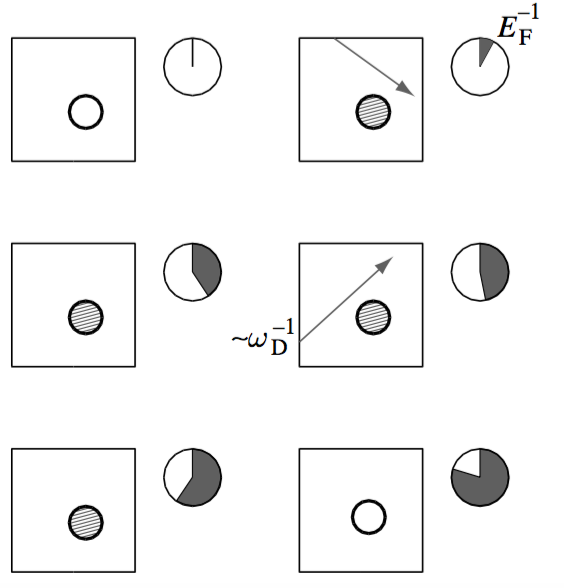
\includegraphics[width=4cm]{./figures/pic1.png}
\caption{Attractive interaction between electrons}
\end{figure}

We can explain this attractive force in a brief way. When an electron moves around an ion, the Coulomb force between them will cause a distortion. Ions move slower than electrons, so after the electron goes far away, the ion still doesn't return its equilibrium position and create a local positive charge density. Another electron will be attracted by this positive charge density.

\section{BCS Hamiltonian and Cooper Pairs}
We now concentrate on the behaviour around the Fermi surface. In Section 2 I have showed that the interaction is attractive when the temperature is lower than Debye frequency. That means the scattering process is limited in a shell with width $\Delta \sim \omega_D$ around the Fermi surface as the following figure shows:
\begin{figure}[!htp]
\centering
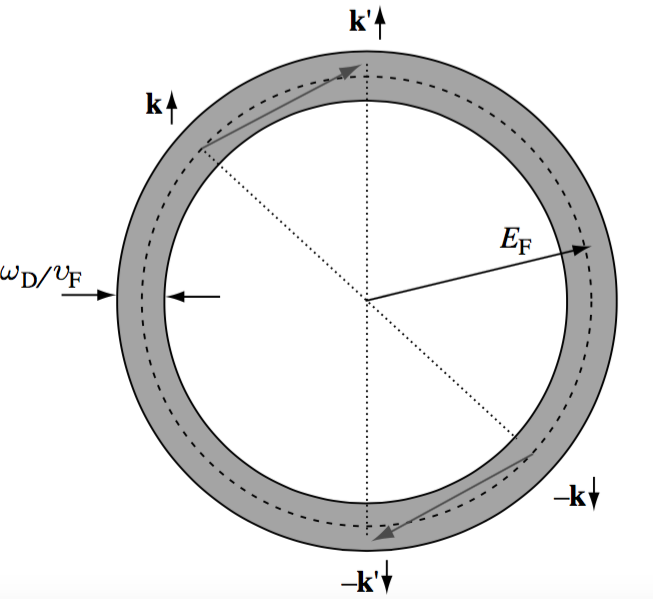
\includegraphics[width = 4cm]{./figures/pic2.png}
\caption{Electrons scattering processes happen in the momentum shell.}
\end{figure}\\
So we can write down an effective Hamiltonian which describes the electron-electron interaction around the Fermi surface:
\begin{equation}
H = \sum_{\mtk}\frac{\mtk^2}{2m}c^\dagger_{\mtk\sigma}c_{\mtk\sigma} - \frac{g}{L^3}\sum_{\mtk\mtk'\mtq} c^\dagger_{\mtk+\mtq\uspin}c^\dagger_{-\mtk\dspin}c_{-\mtk'+\mtq \dspin}c_{\mtk'\uspin}
\end{equation}
in which $g$ is a positive coupling constant with dimension $\mathrm{[energy]^{-2}}$. To analysis the Cooper instability, we can calculate the {\bf{two-particle correlation function}} by summing up all the "ladder diagrams".
\begin{fmffile}{BCSladder}
\begin{equation}
\sum_{\mtk\mtk'}\langle \bar{\psi}_{\mtk\uspin}\bar{\psi}_{-\mtk\dspin}\psi_{-\mtk'\dspin}\psi_{\mtk'\uspin}\rangle= \parbox{30mm}{\begin{fmfgraph}(100,50) \fmfleft{i1,i2} \fmfright{o1,o2} \fmf{fermion}{i1,o1}\fmf{fermion}{i2,o2}\end{fmfgraph}}\quad + \quad \parbox{30mm}{\begin{fmfgraph}(100,50) \fmfleft{i1,i2} \fmfright{o1,o2} \fmf{fermion}{i1,v1,o1} \fmf{fermion}{i2,v2,o2} \fmf{photon,tension = 0}{v1,v2}\end{fmfgraph}}\quad + \quad\parbox{30mm}{\begin{fmfgraph}(100,50) \fmfleft{i1,i2} \fmfright{o1,o2} \fmf{fermion}{i1,v1,v2,o1}\fmf{fermion}{i2,v3,v4,o2}\fmf{photon,tension = 0}{v1,v3}\fmf{photon,tension = 0}{v2,v4}\end{fmfgraph}} \quad + \quad\cdots
\end{equation}
\end{fmffile}
We can find that Eq(12) is the correlation function of Cooper pairs with momentum $q=0$ : $c_{-\mtk\dspin}c_{\mtk\uspin}$. So if the correlation function is divergent at some temperature, that means there will be a phase transition.

Now let's calculate the result of Cooper instability. The calculating process is the following equaitons:
\begin{equation}
C(q=0) =\sum_{kk'} G_k G_{-k}\delta_{kk'} + \sum_{kk'}G_{k}G_{-k}\Gamma_0 G_{k'}G_{-k'}
\end{equation}
and the vertex $\Gamma$ satisfies that
$$
\Gamma_0 = g + g\frac{T}{L^d}\sum_{p}G_{p}G_{-p}\Gamma_0 \quad\Rightarrow\quad \Gamma_0 = \frac{g}{1-\frac{gT}{L^d}\sum_{p}G_p G_{-p}}
$$
So if there is a singularity of vertex $\Gamma_0$, that means a second order phase transition. Now we try to find the precise result of the vertex. First we need to get the result of the summation of Green Functions:
\begin{eqnarray}
\sum_p G_p G_{-p} &=& \sum_{\mtp}\sum_{\omega_m}\frac{1}{-i\omega_m +\xi_\mtp}\frac{1}{-i\omega_m + \xi_\mtp}\nonumber\\
&=& 
\end{eqnarray}

\section{Mean Field Theory at $T = 0\mathrm{K}$}

\section{Mean Field Theory by Path Integral}

\section{Couple to the electromagnetic field}

\section{Anderson-Higgs Mechanism}

\end{document}
